% this file is called up by thesis.tex
% content in this file will be fed into the main document

\chapter{Detecting and Tracking Solar Active Regions} % top level followed by section, subsection
\label{chapter:method_SMART}

% the code below specifies where the figures are stored
\graphicspath{{2/figures/EPS/}{2/figures/}}

%Reset all glossary terms
\glsresetall

%ABSTRACT-----------------------------------------------------
\hrule height 1mm
\vspace{0.5mm}
\hrule height 0.4mm 
\noindent 
\\ {\it 
Most of this chapter is based on research published in \emph{\citetalias{higgins:2011}} and several techniques were first defined in \emph{\citetalias{Verbeeck:2011}}. All of the work presented is mine, except where otherwise noted. In this chapter a system for detecting, characterising, and tracking strong photospheric magnetic features is described and tested. The presented methods are benchmarked by comparing detections to the NOAA active region catalog. The feature characterisation uncertainties resulting from using line-of-sight magnetic field observations are discussed. Good agreement is found between our system and NOAA, but differences are found in feature tracking behaviour, as NOAA's is performed by eye on continuum data and our system is automatically run on magnetic field observations. Finally, to determine the reliability of property determinations, a simulation of a feature crossing the solar disk is used and illustrates that properties incorporating the magnetic gradient incur large errors away from disk center.
}
\\ 
\hrule height 0.4mm
\vspace{0.5mm}
\hrule height 1mm 
\vspace{1.5cm}
%\newpage
%END ABS---------------------------------------------------------

\section{Introduction}

The automatic identification and characterization of solar features is of great importance to both solar activity monitoring and space weather operations. This has become a particular issue due to the high spatial and temporal resolution solar imagers, such as those flown on the \emph{Project for On-Board Autonomy 2} (\emph{PROBA2}) and \emph{Solar Dynamics Observatory} (\emph{SDO}), which will force data providers to distribute subsets of their science products instead of the full image data set. Traditionally, solar feature catalogs were created by hand, using visual recognition to record the position, size, and other properties of features \citep[e.g.,][]{Carrington:1854}. An early attempt to overcome this was SolarMonitor\footnote{See: \url{http://www.SolarMonitor.org}}\citep{Gallagher:2002}, which labels \glspl{AR} in solar images using \gls{NOAA} numbers and locations cataloged by the Space Weather Prediction Center.  More recently, researchers have begun to catalog features using automated methods. The European Grid of Solar Observations\footnote{See: \url{http://www.egso.org}}  \citep[EGSO;][]{Bentley:2002}, for example, catalogs solar features using H$\alpha$ and Ca II K images and a neural network algorithm \citep{Zharkova:2005,ZharkovaSchetinin:2005}. 

One of the first applications of automated image processing techniques to \gls{AR} identification is the Automated Region Selection Extraction algorithm \citep{McAteer:2005a}. This algorithm creates a binary mask of features using a static noise threshold applied to a \gls{LOS} magnetogram. A sub-image is extracted, centered on the pixel with the highest value. Closed contours enclosing an area centered on the seed are grouped as a region. The detected region is saved and removed from the magnetogram. The pixel of the next highest value is selected and the process repeated. Some saved regions are associated with \gls{NOAA} cataloged regions which may be tracked across the disk. More recently,  \citet{LaBonte:2007} extracted \glspl{AR} using full-disk magnetograms that are smoothed by roughly one supergranule diameter. Region candidates are tested for bipolar flux and east-west orientation. A dynamic noise threshold is calculated using the median of average magnetic field values for a series of annuli centered on the \gls{AR} candidate. The \gls{AR} boundary is chosen by comparing the average magnetic field values of smaller annuli with the calculated noise threshold. Using annuli to test for region boundaries allows one to isolate \glspl{AR} from large \gls{AR} complexes since the dynamic noise threshold will be set relative to the surrounding regions.

An alternative to identifying \glspl{AR} solely using their magnetic signatures was discussed in a series of papers by \citet{Qahwaji:2005} and \citet{Colak:2008,Colak:2009}. In their hybrid extraction algorithm, sunspots detected in white-light images are grouped using feature boundaries extracted from magnetograms. Both forms of data are segmented using dynamic thresholding. White-light candidates coinciding with magnetogram candidates are grouped using growing circles, while a neural network is used to determine which candidates to retain and how to group them. This system has the advantage that it compares well the \gls{NOAA} \gls{AR} identification scheme, but it does not give any insight into \gls{AR} properties thought to be related to flaring (e.g., horizontal B-field gradients, total flux, fractal dimension, etc.).

It is known that complicated magnetic field configurations tend to produce more M- and X-class flares than simpler ones \citep{Kunzel:1960,McIntosh:1990}. A number of algorithms have been developed to measure \gls{AR} magnetic characteristics postulated to be related to flaring: \citet{Gallagher:2002} measure gradients in the magnetic field of \glspl{AR}; \citet{mcateer:2005b} establish an \gls{AR} fractal dimension lower limit of 1.2 for M- and X-class flares to occur; \citet{Georgoulis:2007} calculate the magnetic connectivity between fragments of an \gls{AR};  \citet{Conlon:2008,Conlon:2010a} measure the multifractal nature of \gls{AR} flux; \citet{Hewett:2008} determine the multiscale power-law index; and \citet{Falconer:2008} establish a gauge of \gls{AR} non-potentiality.
%; and \citet{Jie:2009} determine basic field properties and the degree of \gls{AR} polarity (bipole, quadrupole, etc.). 
The overall aim of these algorithms is to extract a physically-motivated measure of the characteristics of a region, subsequently using this information to better understand the fundamental physics of \glspl{AR}, and to relate the properties of \gls{AR} magnetic fields to their flaring potential. This is essential to building an automated \gls{AR} monitoring and flare forecasting system as discussed in \citet{McAteer:2009}. 

In this chapter we present a new algorithm, the \gls{SMART}.
%, which will form the basis of \gls{AR} identification for the Heliophysics Integrated Observatory\footnote{See: http://www.helio-vo.org} (HELIO).  
\gls{SMART} combines extraction techniques with \gls{AR} magnetic property determinations (Section~\ref{algorithm}), region tracking, and cataloging (Section~\ref{tracking}). 
%The uncertainties associated with properties measured using \gls{SMART} as well as the results of benchmarking \gls{SMART} against \gls{NOAA} detections are presented in Chapter~\ref{chapter:results_uncert}.
A cross comparison of \gls{SMART} and \gls{NOAA} detections as well as a discussion of errors in property measurements and feature tracking test cases are presented in Section~\ref{sect:smartresults}. Our conclusions are presented in Section~\ref{sect:smartconc}.

\section{Feature Extraction}\label{algorithm}

\begin{figure}[!t]
\centerline{\includegraphics[width=8cm,angle=0]{flowchart_summary.eps}}
\caption[The SMART method.]{Flow chart summarizing the SMART algorithm processing method.}
\label{flowsummary}
\end{figure}

The \gls{SMART} method of operation is summarized in Figure~\ref{flowsummary}. Initially, magnetograms are segmented into individual feature masks (Section~\ref{dataproc}). A characterization algorithm is then run on each extracted region to determine feature properties (Section~\ref{magprop}). These region properties are subsequently used to classify the form of solar features (Section~\ref{classify}).
%Next, features are tracked using consecutive images and through subsequent solar rotations (Section \ref{tracking}). 
The final output is a set of data structures for each magnetogram, including each feature present. The following sub-sections provide details on the operations outlined above.

\subsection{Segmentation}\label{dataproc}

\begin{figure}[!t]
\centerline{\includegraphics[width=10cm,angle=0]{segment_flow.eps}}
\caption[The SMART segmentation method.]{Flow chart summarizing the magnetogram segmentation method.}
\label{segment}
\end{figure}

The segmentation process depicted in Figure~\ref{segment} begins with two consecutive \gls{MDI} full-disk, \gls{LOS}, level 1.8 magnetograms\footnote{See \url{http://soi.stanford.edu/magnetic/Lev1.8/}}. 
%!!! Correction for sensitivity/saturation/ papers...
Nominally these are $96$\,minutes apart, but there are sporadic gaps in the MDI data set (only rarely is there an entire day with no data). We use two magnetograms recorded close in time to remove short-lived features, such as ephemeral flux regions and small bipoles, and to extract time-dependent properties. The magnetogram of interest (Figure~\ref{processing} A) is denoted as $B_{t}$ and the previous magnetogram as $B_{t-\Delta t}$. If $\Delta t$ is greater than one day, the detections are discarded.
%Figure \ref{segment} shows the order of processing steps applied to the data to create the final mask of features present in $B_{t}$. 

\begin{figure}[!t]
\centerline{\includegraphics[width=8cm,angle=0]{processing.eps}}
\caption[Example SMART image processing steps.]{Processing steps for an example feature extraction on 25 November 2003. A) Calibrated magnetogram $B_{t}$ clipped to $\pm$$1\,000$\,G and cropped around NOAA 10507. B) $B_{t}$ with Gaussian smoothing and noise thresholding. C) Mask ($M_{f,t}$) with transient filtering and area threshold of $50$\,pixels. D) Final indexed grown feature mask, $IGM_{t,i}$.}
\label{processing}
\end{figure}

Magnetograms are first checked for problems using properties extracted from the \gls{FITS} data file headers, such as the spacecraft roll angle and the number of missing pixel values. Magnetograms are rotated as necessary, so that solar north points up, using nearest neighbor sampling interpolation, while those with missing values are discarded. A \gls{SEP} event that occurs during a magnetogram exposure results in many bright pixels randomly scattered about the image,. This does not interfere with the \gls{AR} detection, as the bright pixels are smoothed out and not detected as an AR, but can affect magnetic property determinations. %This is discussed in Section \ref{results}.

We first apply smoothing, a noise threshold, and a magnetic field \gls{LOS} correction, respectively, to the data (Figure~\ref{processing} B). This set of operations is represented by \emph{STL Process} in Figure~\ref{segment}. The smoothing operation is necessary to remove ephemeral regions that have size scales on the order of $10$\,Mm \citep{Hagenaar:2001}, which corresponds to $7$~MDI~pixels at disk center.
%and network bright points (which are smaller)!!!ref??. 
To this end, $B_{t-\Delta t}$ and $B_{t}$ are convolved with a $10\times 10$\,pixel$^2$ kernel containing a 2D gaussian with a full-width at half-maximum (FWHM) of $5$\,pixels, which is sufficient to avoid detecting them. A 2D boxcar smoothing was also attempted, but resulted in linear artifacts in the final detections.

\begin{figure}[!t]
\centerline{\includegraphics[width=12cm,angle=0]{mdi_quiet_stddev_maxb_vs_cycle100x100_sm1_bth100.eps}}
\caption[Maximum QS magnetic field over the solar cycle.]{The maximum of quiet-Sun magnetic field values over solar cycle 23. Each point is the mean maximum value for a month of magnetograms (nominally two per day are used, but less for particularly active periods). The vertical bars indicate the spread of values using the standard deviations of each month's set of values. The green line indicates the mean of the monthly mean values. The continuous gray line is the smoothed, monthly sunspot number from Solar Influences Data Analysis Center (SIDC; \url{http://sidc.oma.be}).}
\label{cycle_sig}
\end{figure}

\begin{figure}[!t]
\centerline{\includegraphics[width=10cm,angle=0]{mdi_qs_arbeta_sm1.eps}}
\caption[AR magnetic field distribution.]{A comparison of magnetic field value distributions for a quiet-Sun and solar feature region. \emph{Top left}: Magnetogram of NOAA 8086, gaussian smoothed using a FWHM of 5\,pixels. \emph{Top right}: A nearby region of quiet Sun in the same full-disk image. \emph{Bottom}: The feature and quiet-Sun unsigned magnetic field distributions. The thick red line is the difference between the quiet-Sun and AR distributions and the vertical dash-dotted line denotes $70$\,G.}
\label{ar_qs_dist}
\end{figure}

We use a static threshold of $\pm$70\,G to remove the background. Figure~\ref{cycle_sig} shows the variation in the monthly averages of maximum values of \gls{quietsun} (QS) magnetic field recorded throughout cycle 23. The maximum value varies by roughly $5$\,G over the cycle which is less than the monthly standard deviation of these maxima. The mean of the maximum unsigned \gls{quietsun} magnetic field values is $\sim$$70$\,G. 

Degradation in the MDI instrument may contribute to a portion of the variability seen in these mean values over the solar cycle. \cite{Liu:2004} find a random offset in MDI magnetogram values that varies between $\pm$2\,G due to noise resulting from the camera shutter. The maximum magnitude of the offset appears to increase from $\sim$1 to $\sim$1.5 between the period 1997 to 2001. In \cite{Schou:2004} a measure of charge leakage in the CCD is determined for the period of 1996\,--\,2004. This increases by $\sim$25\% during 1996\,--\,2002 and then levels off and decreases slightly in 2003\,--\,2004. It is not indicated how charge leakage affects measured field values. The quiet-Sun magnetic field values peak at solar maximum and show minima at solar minimum. Without considering these instrumental errors, this is explained by the greater amount of emerging and decaying flux observed on disk that contributes to the background quiet-Sun. Using a static threshold results in more or less background flux being included in a given detection, depending on the phase of the solar cycle.

Figure~\ref{ar_qs_dist} shows a smoothed \gls{AR} and nearby \gls{quietsun} region contoured at $\pm$$70$\,G. The histogram shows the distributions of magnetic field values for the \gls{AR} and \gls{quietsun} regions, including the difference between the two distributions. Thresholding at the  $\pm$$70$\,G level removes small features which have been smoothed out by the gaussian convolution but maintains extended strong-field features, such as bipolar and plage regions. Pixels in $B_{t-\Delta t}$ and $B_{t}$ with absolute values less than $70$\,G are zeroed.

In the case where magnetic fields are primarily normal to the solar surface, the \gls{LOS} component of the field is reduced toward the limb. This does not hold for sunspot penumbrae, as discussed in Section\,\ref{sect:quantmagfield}. As such, a feature with the same magnetic field strength and orientation with respect to the solar surface will appear lower in magnitude when located toward the solar limb than at disk center. This \gls{LOS} effect is corrected at each \gls{MDI} pixel using a cosine correction factor. This method results in detections that include sunspot penumbrae having lower total magnetic flux values, due to their non-normal fields. % \citep{McAteer:2005a}.
%The LOS effect is corrected at each MDI pixel using \citep{McAt05}, 
%\begin{equation}\label{eqn_ardata}{%
%	B=\frac{B_{0}}{\sin(\arccos( r/r_{sun} ) ) }
%}
%\overfullrule 5pt
%\mathindent\linewidth\relax
%\advance\mathindent-259pt
%\end{equation}
%where $B_{0}$ is the measured field magnitude, B is the corrected value, $r$ is the pixel's heliocentric radial distance from disk center and $r_{sun}$ is the heliocentric (plane-of-sky) radius of the sun. 
After this stage, $B_{t-\Delta t}$ data is differentially rotated to time $t$ to correct for feature motions due to solar rotation using the latitudinal dependence derived in \citet{Howard:1990}.

\begin{table}[!t]
\centerline{\begin{tabular}{lcl}
\hline
Data Type&Identifier&Explanation\\
\hline
Feature Array&$B_{t,i}$ & extracted feature magnetogram \\
&$IGM_{t,i}$ & extracted feature mask \\ 
&$HG_{t}$ & heliographic position map \\
%$HC_{t}$ & map of heliocentric positions for each region pixel \\ 
&$A_{cos,t,i}$ & $ \frac{IGM_{t,i}}{ \cos(HG_{t}} \times (\mbox{1.4 Mm}^{2}/\mbox{pixel})^{-1}$ \\
&${\Phi}_{t,i}$ & $B_{t}\times A_{cos,t,i}$ \\
&${\frac{d\Phi}{dt}}|_{t,i}$ & $\frac{(\mid B_{t}\mid - \mid B_{t-\Delta t}\mid )\times A_{cos,t,i}}{\Delta t}$\\
\hline
Property Value&$HG_{pos,t,i}$ & $\frac{\sum_{pix} ({B_{t,i}\times HG_{t}})}{\sum_{pix}{(HG_{t} \times IGM_{t,i})}}$ \\
&$B_{max,t,i}$ & maximum value of $B_{t,i}$ \\
&$B_{min,t,i}$ & minimum value of $B_{t,i}$ \\
&$B_{tot,t,i}$ & $\sum_{pix} {B_{t,i}}$ \\
&$B_{tot\mbox{ }uns,t,i}$ & $\sum_{pix} {\mid B_{t,i}\mid}$ \\
&$\mu,\sigma^2,\gamma,\kappa$ & mean, variance, skewness, kurtosis \\
&$A_{tot,t,i}$ & $\sum_{pix} A_{cos,t,i}$ \\
&${\Phi}_{+,t,i}$ & $\sum_{pix} {({\Phi}_{t,i}>0)}$ \\
&${\Phi}_{-,t,i}$ & $\sum_{pix} {({\Phi}_{t,i}<0)}$ \\
&${\Phi}_{uns,t,i}$ & $\sum_{pix} {\mid {\Phi}_{t,i}\mid}$ \\
&${\Phi}_{imb,t,i}$ & $\frac{\mid({\Phi}_{+,t,i}-\mid {\Phi}_{-,t,i}\mid )\mid }{ \Phi_{uns,t,i}}$ \\
&$\frac{d\Phi}{dt}|_{net,t,i}$ & $\sum_{pix} {{\frac{d\Phi}{dt}}|_{t,i}}$ \\
\hline
\end{tabular}}
\caption[List of magnetic properties.]{Feature magnetic properties derived from characterization processing.}
\label{tablemagprop}
\end{table}

The corrected magnetograms are made binary by setting all pixels with magnetic field values above the $\pm$$70$\,G threshold equal to one, yielding masks $M_{t-\Delta t}$ and $M_{t}$. This thresholding is the initial segmentation of the magnetogram into separate features. Features consisting of less than $50$\,pixels and those which are not present in both masks are removed by the following operations (Figure~\ref{processing} C). Firstly, each mask is dilated by $10$\,pixels to allow for region expansion between consecutive images. This means that each detected boundary is expanded radially. 

Secondly, the binary masks are subtracted such that non-zero pixels in the difference mask identify features only occurring in $M_{t-\Delta t}$ or $M_{t}$. These transient features are subsequently removed from the un-dilated version of $M_{t}$, which is then dilated by $10$\,pixels to form $M_{f,t}$ (Figure~\ref{processing} D). Individual contiguous features in $M_{f,t}$ are indexed by assigning ascending integer values (beginning with one) in order of decreasing feature size. This indexing is indicated by the subscript $i$ in array and property variables and means that the variable corresponds to a specific feature, rather than the entire solar disk.  The segmentation output is an indexed grown mask ($IGM_{t}$), as shown by the thick red box in Figure~\ref{segment}. The $IGM_{t}$ for a given feature is shown in Figure~\ref{processing} D.


\subsection{Characterization}\label{magprop}

\begin{figure}[!t]
\centerline{\includegraphics[width=12cm,angle=0]{characterize_flow.eps}}
\caption[The SMART characterisation method.]{Flow chart summarizing the feature magnetic property characterization method.}
\label{flow_char}
\end{figure}

The aim of \gls{SMART} is to characterize \glspl{AR} in a manner which does not make many theoretical assumptions (except for the assumption that magnetic fields are normal to the solar surface) or require many observations of the same feature.  Our design is adaptable, so that the software may produce initial results in near-realtime for operational purposes, but allows the retrospective addition of complex property measurements (e.g., magnetic helicity). These requirements define criteria for the selection of initial property calculations. There are many \gls{AR} properties that may be derived from magnetograms. A subset of these are derived from 96 minute \gls{LOS} data and those output by \gls{SMART} are included in Tables\,\ref{tablemagprop} and \ref{tablehighorder}. Not all of the properties listed here are investigated in this thesis, but they are included presently to act as a reference for other work \citep[e.g.][]{Ahmed:2011}.

The \gls{SMART} characterization process utilizes the feature mask ($IGM_{t}$) retrieved by the methods outlined in the previous section, following the procedure detailed in Figure~\ref{flow_char}. This mask contains all of the features visible on the solar disk at a given time. The property measurements are derived from the magnetogram taken at time, $t$ which is processed in the manner detailed below. We subscript the mask containing all features by $i$ to extract a single feature mask, $IGM_{t,i}$. A cosine-corrected pixel-area map, $A_{cos,t,i}$,  is constructed that contains pixel areas corrected to solar surface area rather than plane-of-sky area, and is summed to yield total feature area, $A_{tot,t,i}$. 

\begin{table}[!t]
\centerline{
\begin{tabular}{lcl}
\hline
Data Type&Identifier&Explanation\\
\hline
Feature Array&$M_{PSL,t,i}$ & polarity separation line mask \\
&$M_{PSL,thin,t,i}$ & thinned polarity separation line mask \\
\hline
Property Value&$L_{PSL,t,i}$ & $\sum_{pix}{M_{PSL,thin,t,i}}$ \\
&$L_{sg,t,i}$ & $L_{PSL,t,i} > 50$\,G\,Mm$^{-1}$ \\
&$R_{t,i}$ & $R$-value: flux near a PSL \\ %\tnote{1}\footnotemark[1] \\
&$R^{*}_{t,i}$ & $\sum_{pix}{(M_{PSL,t,i} \ast Gauss_{2D})\times B_{t,i}} $ \\
&$WL_{sg,t,i}$ & non-potentiality gauge \\ %\tnote{2}\footnotemark[2]\\
&$WL^{*}_{sg,t,i}$ & $\sum_{pix}{M_{PSL,t,i} \times \nabla B_{t,i}} $ \\
\hline
\end{tabular}}
\caption[A list of PSL-related physical properties.]{Feature magnetic properties derived from polarity separation line characterization.}
\label{tablehighorder}
\end{table}

%\begin{threeparttable}
%\begin{tablenotes} \footnotesize
%\item[1] Schrijver (2007)
%\item[2] Falconer \emph{et al.} (2008)
%\end{tablenotes}
%\end{threeparttable}}
%\protect\citet{Schrijver:2007}
 %\protect\citet{Falconer:2008}
%\footnotetext[1]{\citet{Shj07}}
%\footnotetext[2]{\citet{Fal08}}


Full-disk magnetograms $B_{t-\Delta t}$ and $B_{t}$ are processed as in Section \ref{dataproc} (thresholding, LOS correction, $B_{t-\Delta t}$ differentially rotated to time $t$), but without smoothing. Single features are extracted for magnetic property determination using the indexed grown mask,
\begin{equation}\label{eqn_ardata}{%
    B_{t,i} = {IGM_{t,i}} \times {B_{t}} \mbox{ \ ,}
}
\overfullrule 5pt
%\mathindent
%\linewidth
%\relax
%\advance
%\mathindent -259pt
\end{equation}
yielding an array where all pixels but those in the feature are set to zero. 
The processed magnetograms  are subtracted and divided by their time separation to yield a map of the temporal change in field strength, ${{dB}/{dt}}|_{t}$, leading up to time $t$. This is combined with $A_{cos,t,i}$ to determine the flux emergence rate, ${{d\Phi}/{dt}}|_{t,i}$, of feature $i$.

\begin{figure}[!t]
\centerline{\includegraphics[width=10cm,angle=0]{highorder_flow.eps}}
\caption[SMART characterisation method for PSLs.]{Flow chart summarizing the quantities derived from feature polarity separation lines.}\label{flow_highorder}
\end{figure}

The extracted $B_{t,i}$ is used to extract other properties from feature $i$ (as detailed in Table\,\ref{tablemagprop}) such as statistical moments of the magnetic field and the minimum and maximum magnetic field values ($B_{min,t,i}$ and $B_{max,t,i}$). $B_{t,i}$ is multiplied by $A_{cos,t,i}$ to derive the total positive, negative, and unsigned flux (${\Phi}_{+,t,i}$, ${\Phi}_{-,t,i}$, and ${\Phi}_{uns,t,i}$), the relative flux imbalance (${\Phi}_{imb,t,i}$), and the net flux emergence rate (${{d\Phi}/{dt}}|_{net,t,i}$).

\begin{figure}[!t]
\centerline{\includegraphics[width=8cm,angle=0]{classify_flow.eps}}
\caption[The SMART classification method.]{Flow chart summarizing the feature classification method.}
\label{flow_class}
\end{figure}

The extracted feature magnetogram, $B_{t,i}$, is also used to derive properties based on the \gls{PSL}. Figure~\ref{flow_highorder} summarizes the extraction of feature properties related to \glspl{PSL} and Table\,\ref{tablehighorder} lists the properties derived. Initially, the feature is segmented into its positive and negative components. These components are used to create a positive and negative mask, each of which is dilated by $4$\,pixels. The two masks are summed and the region of mask overlap becomes the \gls{PSL} binary mask, $M_{PSL,t,i}$. The algorithm then thins\footnote{Thinning is done using a morphological algorithm including a sequence of erosions using specific kernals. The IDL M\_THIN routine is used, as described on page 25 of \url{http://www.cis.rit.edu/class/simg782/lectures/lecture_04/lec782\_05\_04.pdf}} $M_{PSL,t,i}$ to a single pixel width ($M_{PSL,thin,t,i}$) and sums the non-zero pixels to determine the \gls{PSL} length ($L_{PSL,t,i}$).  $L_{sg,t,i}$ is obtained by summing only those pixels which have $\nabla B_{t,i} > 50$\,G\,Mm$^{-1}$, where $\nabla B_{t,i}$ is calculated by numerical differentiation using 3-point Lagrangian interpolation. 

We also calculate the \gls{rvalue} ($R_{t,i}$) as presented in \citet{Schrijver:2007} and the \gls{wlsg} gauge ($WL_{sg,t,i}$) as presented in \citet{Falconer:2008}. \gls{rvalue} is the amount of total flux near a \gls{PSL} and \gls{wlsg} is the sum of the gradient along a \gls{PSL}. Both of these use specific gradient and magnetic field thresholding when extracting the \gls{PSL}. These measures are important for flaring, as shown by the investigation in Chapter\,\ref{chapter:results_activity}. Using $M_{PSL,t,i}$ we calculate $R^{*}_{t,i}$ which is a more sensitive version of the \gls{rvalue}, since it contains no gradient thresholding and the magnetic field threshold of $\pm$$70$\,G is much lower than the $\pm$$150$\,G used in \citet{Schrijver:2007}. The algorithm convolves $M_{PSL,t,i}$ with a $20\times20$\,pixel$^2$ kernel containing a 2D gaussian with a FWHM of $10$\,pixels, which is multiplied by $B_{t,i}$ and summed to achieve $R_{t,i}^{*}$. Similarly, an alternative of $WL_{sg,t,i}$, $WL^{*}_{sg,t,i}$ is calculated by applying the \citet{Falconer:2008} method, but using a magnetic field threshold of $\pm$$70$\,G and no gradient threshold. The measures, $R^{*}_{t,i}$ and $WL^{*}_{sg,t,i}$ are useful for characterising small, weak, or emerging features that may not have developed strong PSLs and may have $R_{t,i}$ and $WL_{sg,t,i}$ values equal to zero.

A set of data structures is created for each magnetogram including the above mentioned properties of each extracted feature (used for classification; Section~\ref{classify}) and the feature's heliographic location and time of measurement (used for feature tracking; Section~\ref{tracking}).


\subsection{Secondary Characterisation Modules} \label{sect:char2}

\begin{figure}[!t]
\centerline{\includegraphics[width=0.9\textwidth,clip=]{smartbipolepslexamp.eps}}
\caption[Example PSL and Ising energy determination.]{Left: NOAA 10365 highlighting the PSL (white contour), a linear fit to the locus of PSL positions (dotted red line), bipolar
connection line (solid red line),
and heliographic longitude and latitude reference lines (dotted black lines). Right: An
Ising energy map of
the same region. Red represents the magnitude of energy for each pixel from
highest (light) to lowest (dark). Since the connection between pixels of
opposite polarity is being represented, the energy map is only shown for one of
the polarities.}
\label{smartbipolepslexamp}
\end{figure}

Several auxiliary physical property modules have been designed, used in their original form, or adapted and run on \gls{SMART} detections for the investigations presented in Chapter~\ref{chapter:results_activity}. The modules measure the orientation of the sunspot group magnetic polarities, a proxy for multi-scale energy distribution, and proxies for the magnetic interconnectivity of magnetic elements within a sunspot group. While these properties are not linearly independent as they are all related to polarity mixing, used in conjunction they give a more reliable picture of the evolution of sunspot group magnetic fields.

The tilt of a sunspot group is obtained by measuring the angle between the line connecting the centroids of the positive and negative blobs of largest flux (solid red line in left panel of Figure \ref{smartbipolepslexamp}) and the heliographic latitude line passing through the centroid of the sunspot group. The length of this \gls{BCL} line is also  determined and provides a measure of relative compactness when compared to the evolution of total area (left panel of Figure \ref{smartbipolepslexamp}). Additionally, the angle ($\alpha$) detected between the best-fit line to the locus of pixels forming the main \gls{PSL} and the \gls{BCL} is measured. The main \gls{PSL} is defined as that separating the aforementioned largest flux-weighted positive and negative blobs. The temporal derivative of the angle $\alpha$ is shown to be a useful proxy for the occurrence of helicity injection \citep{Morita:2005}, which may be an important flare predictor \citep{LaBonte:2007}. The evolution of this angle is studied in Chapter~\ref{chapter:results_activity}. 

These properties are less informative when studying sunspot group complexes or non-bipolar groups, since often no main axes can be discerned, making a description of the group's orientation impossible. Complexes are often highly flare-productive, so an assessment of separate regions within a single complex would be useful. This could be done by dividing up a complex into constituent regions using the more compact white-light signatures of sunspots.

%A proxy for complexity used in this work relies on wavelets to determine a scale power spectrum. The wavelet transform of a magnetogram image at scale $a$ is the convolution of the Marr wavelet with an image,
%\begin{equation}
%\omega_a = \phi_a * I \mbox{\,,}
%\end{equation}
%and the energy at each scale is given by, 
%\begin{equation}
%E(a) = \frac{1}{c} \int |\omega_a(x)|^2 dx \mbox{\,,} 
%\end{equation}	
%where $c$ is the admissibility constant. The evolution of the slope of this energy spectrum is determined in this work. this has been shown to be related to flaring in several case studies \citep{Hewett:2008}. 
Here, the complexity of sunspot groups is defined by the mixing of opposite polarities. A bipole is considered less complex than a group with a quadrupolar configuration. Since magnetic connectivity is thought to be depend on the distance between regions of opposite polarity, it is used to indicate complexity. The magnetic free-energy available for flaring is thought to be larger in more interconnected and complex sunspot groups\citep{Schrijver:2009,Falconer:2009,Georgoulis:2007}. The properties used in this work as proxies for inter-connectivity and complexity in sunspot groups, ``B-effective"  \citep[$B_{eff}$;][]{Georgoulis:2007} and Ising energy \citep{Ahmed:2010}, are known to be related to flare productivity. Large values of either one have been shown to indicate the flare productivity of a sunspot group. The calculation of each is explained in depth in the original papers but a summary is given here. 

To calculate $B_{eff}$ simulated annealing\footnote{Simulated annealing is a method of iteratively searching for a solution by minimising some function. The process is halted once the function returns a stable result.} \citep{Press:1992} is used to determine the connections between flux elements (each can be connected to two other elements), which simultaneously minimizes the distance between those elements and the flux imbalance in a magnetic region, 
\begin{equation}
F=\sum^m_{i=1} \sum^l_{j=1} \left( \frac{|r_i-r_j|}{|r_i|+|r_j|} + \frac{\phi_i^{'}+\phi_j^{'}}{|\phi_i^{'}| + |\phi_j^{'}|} \right) \mbox{\,.}
\end{equation}
Then,
\begin{equation}
B_{eff}=\sum^m_{i=1} \sum^l_{j=1} \frac{\phi_{ij}}{L^2_{ij}} \mbox{\,, for } \phi_{ij} \neq 0 \mbox{,}
\end{equation}
where the ratio of the net flux and distance between each connected element is summed over all elements. 

Finally, Ising energy is determined in a similar way, but instead of using a minimization technique, the product of magnetic field values divided by the square of the distance between them is summed for all possible connections. Here we use a modified form of the equation given by \citet{Ahmed:2010}. The version used in this work is calculated using,
\begin{equation}
\displaystyle\sum\limits_{i,j} \left|\frac{B_i B_j}{D_{ij}}\right| \mbox{,} 
\end{equation}
where $B_i$ ($B_j$) are pixel values of positive (negative) line-of-sight magnetic field and $D_{ij}$ is the spatial distance between pixels $i$ and $j$. The Ising energy increases as the negative and positive magnetic footprints within an active region become more entangled. 


\subsection{Classification}\label{classify}

\begin{figure}[!t]
\centerline{\includegraphics[width=0.9\textwidth,clip=]{smart_20031029_1115.eps}}
\caption[An example set of classified SMART detections.]{The set of SMART detections for 29 October 2003. Classifications for each detection are shown by the black labels. The detection types shown include AR (large multipolar), PL (large unipolar), and DF (small decaying unipolar).}
\label{smartexampledetections}
\end{figure}

At this stage the \gls{SMART} algorithm has characterized the properties of each automatically extracted feature. The classification process uses these properties to discriminate between various feature types, which are saved in the algorithm output. Extracted features are initially grouped (as shown in Figure~\ref{flow_class}) into two catagories: 
%%We use a flux imbalance threshold of 90\% to distinguish unipolar features.
features with a flux imbalance (as defined in Table\,\ref{tablemagprop}) greater than 90\% are classified unipolar (U), while those having less than 90\% are classified multipolar (M). The 90\% threshold chosen is arbitrary and is not 100\% to allow for small features of the opposite polarity to merge with the main feature and not change its classification to multipolar. After polarity balance, the total unsigned magnetic flux ($\Phi_{uns,t,i}$) is tested. Features with $\Phi_{uns,t,i}$ greater than $10^{21}$\,Mx are classified as big (B), while features with $\Phi_{uns,t,i}$ less than $10^{21}$\,Mx are classified as small (S).
%Unipolar features with $\Phi_{uns,t,i}$ greater than $10^{21}$\,Mx are classified as plage (PL), while multipolar features with $\Phi_{uns,t,i}$ greater than $10^{21}$\,Mx are classified as potential \glspl{AR}.
%%Plage regions must have a total unsigned magnetic flux of at least $10^{21}Mx$. Features having less flux than this are determined to be long lifetime ephemeral regions \citep{HH01} or fragmented plage regions. Multipolar features are required to have a flux imbalance of less than 10\%. 
%Features having an unsigned magnetic flux below $10^{21}$\,Mx are 
%labeled as either emerging regions (ER) if they are growing in magnetic flux or decaying regions (DR) if their magnetic flux is decreasing.
Finally, the sign of ${\frac{d\Phi}{dt}}|_{t,i}$ is tested to determine if features are increasing in flux (emerging, E) or decreasing in flux (decaying, D).  This should indicate changes occurring over the dynamic time-scales of sunspot groups rather than those due to rotation on or off the solar disk, since the difference in flux is determined between consecutive images (nominally 96\,minutes). The classification scheme results in eight possible feature classifications which are then also attributed to common magnetic feature designations: MBE and MBD are denoted evolving \glspl{AR}; MSE and USE are denoted emerging flux concentration (EF); MSD, USD, and are denoted decaying flux concentrations (DF), and finally, UBE and UBD are denoted plage (PL). Plage can be described by extended unipolar regions of magnetic flux (see Section\,\ref{sect:sunspots}), and so is used as a designation here. These common designations are also saved in the algorithm output, allowing one to make a quick assessment of which regions on disk are interesting from a monitoring point of view. For example, EFs may become \glspl{AR} and evolving \glspl{AR} may produce activity during their evolution, while PL and DF are not likely to produce activity. An example set of classified detections is shown in Figure\,\ref{smartexampledetections}.

\section{Tracking}\label{tracking}

Having detected various solar features, the \gls{SMART} algorithm associates features across different time intervals. 
Spatial and temporal information is used to track features between consecutive images (Section~\ref{history}) and around the far-side of the disk between consecutive solar rotations (Sections~\ref{history2}). Features are then cataloged using the time of their first detection and their classification (Section~\ref{cataloging}). 

\subsection{Consecutive Images}\label{history}

The set of features in a magnetogram is compared with the previous five magnetogram sets to associate previously catalogued features with the current set. Feature positions ($HG_{pos,t,i}$) are differentially rotated, using the latitudinal dependence of the rotation rate derived in \citet{Howard:1990}, to the same time $t$ and features matched when their heliographic centroid separations are less than $5^\circ$. Features having one classification in previous sets may be associated with features having a different one in the current set. Thus, the \gls{SMART} algorithm is capable of tracking possible \glspl{AR} (MBE, MBD) back to their first emergence as an EF (MSE). Decaying features may also be associated with features previously denoted as possible \glspl{AR}, allowing \glspl{AR} to be followed through their final stages of evolution.
%Then we  match features in the previous solar rotation as described in Section~\ref{history2}. 
%At this point, regions classified as \gls{AR} or PL which have yet to be cataloged are given a name using the convention described in Section \ref{cataloging}.
Fragmentation often occurs in these late stages which \gls{SMART} allows for since it does not preclude multiple features from being associated with a single previous feature. If one feature splits into two, each resulting fragment will be associated with the original feature if the resulting fragment positions are within the matching centroid-separation threshold of the original. A letter is appended to the catalog name of each additional associated feature so that individual fragments may be differentiated. 
%This is shown in Figure~\ref{detectcases}.
%!!! INSERt REF!!!

\subsection{Far-side Passage}\label{history2}

Features are tracked beyond the limb through multiple solar rotations to study their evolution from emergence to decay. We calculate the rotation period, $P_{rot,i}$, for each feature at time $t$, which depends on its heliographic latitude due to differential solar rotation. The feature position is compared to those in the five magnetogram sets centered on time $(t+t_{70})-P_{rot,i}$ using the method in the previous section, where $t_{70}$ is the time taken for the feature to rotate to $70^{\circ}$ heliographic longitude from its position at $t$. In this approach the feature position is essentially rotated to a longitude of $+70^{\circ}$ then back one full solar rotation. In this way the feature is constrained to have been previously detected just before west limb passage, which increases the efficiency of the algorithm.

\subsection{Cataloging}\label{cataloging}

There are two identifications recorded for each detected feature in a magnetogram at time, $t$. The first, $i$ is an index number that uniquely identifies the feature within a magnetogram and is obtained from $IGM_{t}$. The index number, $i$, also denotes the two-digit size order of the feature. The second identification is the static catalog name, YYYYMMDD.MG.NN, where YYYY is the four digit year, MM is the two digit month, and DD is the two digit day. The next two characters specify the feature type: MG denotes a photospheric magnetic feature and represents any SMART detections. This scheme can be expanded to incorporate coronal holes (CH), filaments (FI), and transient features such as flares (FL) and coronal mass ejections (CE) in EUV images. Finally, NN is $i$ when the feature is given a static catalog name. This catalog name is determined once for each feature upon first detection, and is used for all measurements of the same feature as it is tracked through time. 


%%%%%%%%%%%%%%%%%%%%%%%%%%%%%%%%%%%%%%%%%%%%%%%%%%
\section{Results and Discussion}\label{sect:smartresults}
%%%%%%%%%%%%%%%%%%%%%%%%%%%%%%%%%%%%%%%%%%%%%%%%%%

In this section we investigate the uncertainties involved in characterising the magnetic fields of sunspot groups using \gls{LOS} photospheric magnetograms. The material presented in Section~\ref{sect:smartmethuncert} is from \cite{higgins:2011} The finite resolution of the observations limits what can be said about the magnetic field magnitude, regardless of the method used to measure it (Section~\ref{sect:fillfact}). Uncertainties due to the method used to detect and characterise sunspot groups are manifested in the stability of tracked detections (Section~\ref{sect:smartmethuncert}). These uncertainties are investigated further by simulating a feature on the solar surface and tracking its measured properties over time (Section~\ref{sect:simuncert}).

Some calibration issues with the \gls{MDI} data used by \gls{SMART} are discussed in \citet{Wang:2009}. It was found that the 2008 calibration of level 1.8 data has been partially corrected, in that it does not suffer from a disk center-to-limb variation like the 2007 calibration \citep{Tran:2005}. However, \gls{MDI} may largely underestimate the magnetic field as the ratio of \gls{MDI} values to those retrieved from \emph{Hinode}/Solar Optical Telescope data was found to be $\sim$$0.7$. This does not affect feature detections since the effect is consistent throughout the data set, but could contribute a considerable error of $\sim$$30\%$ for any magnetic field or flux measurements. The data used in this work are level 1.8 data.

Strong magnetic field saturation in \gls{MDI} data is discussed in \citet{Liu:2007}. It is estimated that this phenomenon occurs in $\sim$$5\%$ of sunspot groups, in which the magnetic field measurements in the umbral areas of very strong sunspots behave non-linearly. In extreme cases, the umbra may appear to have a smaller magnetic field than the surrounding \gls{penumbra}. In reality, the field should continue to increase in the \gls{umbra}, but in level 1.8 data showing \gls{NOAA} 9002 at disk center, saturation is clearly observed at $\sim$$3\,000$\,G. Feature boundaries are not affected because saturation only occurs for very strong sunspot \glspl{umbra}, although the derived magnetic properties of features which include strong sunspots will be underestimated. 

Another issue with using \gls{MDI} magnetograms is the geometrical effect due to the use of \gls{LOS} fields. As sunspots progress toward the limbs, the apparent magnetic field of the limb-ward penumbra can change polarity. Since \glspl{penumbra} are close to horizontal, their field vector can dip below the plane perpendicular to the \gls{LOS}, causing false \gls{PSL} to emerge. This causes large errors in any property determination related to magnetic field gradient, such as \gls{PSL} length.

\subsection{Magnetic Filling Factor}\label{sect:fillfact}

\begin{figure}[!t]
\centering{\includegraphics[width=0.6\textwidth,angle=0,clip=0]{uncert/fluxtubeschem.eps}}
\caption[A flux-tube observation schematic.]{A schematic of an observation of a vertical flux-tube at the solar surface.}\label{fig:ftschem}
\end{figure}

When imaging the solar surface, the smallest feature that can be defined is limited both by the size of a single pixel and the size of the telescope aperture. This due to the smearing effect of  light diffraction within the telescope. There may be additional effects on the observed signal\footnote{These effects are included in the instrument's point spread function (PSF), which indicates the spatial spread of an observed point source.}, resulting from other elements of the instrument design that are not well characterised in the literature. The optimum pixel size is the theoretical optical resolution\footnote{The best achievable optical resolution of a telescope is $1.22\lambda/D$, where $\lambda$ is wavelength and $D$ is the diameter of the telescope aperture.} divided by 2.3, and is derived using the Nyquist theorem. For MDI, the pixel size is $\sim$4 times that of the optimal pixel size \citep{Schou:2012}, so the effect of diffraction should be negligible. HMI has a pixel size $\sim$30\% larger than the optimal size, so HMI should not be strongly affected by diffraction. 
%http://www.mcb.arizona.edu/IPC/zoom_Page.htm
%http://en.wikipedia.org/wiki/Point_spread_function#The_PSF_in_astronomy

Consider a vertical magnetic \gls{fluxtube} at disk center imaged by a magnetograph. It is likely that strong magnetic fields are bound into \glspl{fluxtube} on the solar surface, so the magnetic field outside of them should be small in comparison. To simplify the problem we assume its magnetic field, $B_{FT}$, is constant over its cross-section. In reality the magnetic field must drop off at the edges of a flux tube since the field must be continuously differentiable. If the \gls{fluxtube} cross-section perfectly fills the magnetograph resolution element, then the magnetic field measurement of the \gls{fluxtube} has a filling factor of 1. In general the filling factor is given by,
\begin{equation}
f \equiv A_{F}/A_{px} \mbox{\,,}
\end{equation}
where $A_{F}$ is the cross-sectional area of a magnetic surface feature within a pixel and $A_{px}$ is the area of a pixel. A schematic of this is shown in Figure~\ref{fig:ftschem}.

\begin{figure}[!t]
\centering{
\includegraphics[width=0.5\textwidth,angle=0,clip=0]{uncert/fluxobspxschem.eps}
}
\caption[A schematic comparison between actual and observed flux-tubes.]{A schematic comparison between the actual configurations of flux-tubes in a pixel and what is observed. When two flux elements of equal area and field strength are present within a pixel, the observed field is 0.}
\label{fig:ftschem2}
\end{figure}

The magnetic field measured, $B_{OB}$, is the average over a pixel. When $f < 1$, $B_{OB}$ is between $B_{F}$ and a presumably lower \gls{quietsun} field of the same polarity, $B_{QS}$. Thus,
\begin{equation}
B_{OB}=f B_{FT} + (1-f)B_{QS} \mbox{\,.}
\end{equation}
While the observed magnetic field is strongly dependent on $f$, flux is less so, depending on $B_{QS}$. Flux is given by,
\begin{eqnarray}
\Phi_{FT} = A_{FT} B_{FT} \mbox{\,,} \\
\Phi_{OB} = A_{px} B_{OB} \mbox{\,,}
\end{eqnarray}
where $\Phi_{FT}$ is the flux of the \gls{fluxtube} within a pixel and $\Phi_{OB}$ is the observed flux in a pixel. The measured flux will then be overestimated due to the \gls{quietsun} contribution. However, if we assume that $f/(1-f) >> B_{QS}/B_{FT}$, then $\Phi_{FT} \approx \Phi_{OB}$ since,
\begin{eqnarray}
\Phi_{OB} &=& A_{px} [f B_{FT} + \underbrace{(1-f)B_{QS}}_{\mbox{negligible}}] \\
 &\approx& A_{px} f B_{FT} \\
 &=& A_{px} \left( \frac{A_{FT}}{A_{px}} \right) B_{FT} \\
\Phi_{OB} &\approx& A_{FT} B_{FT} = \Phi_{FT} \mbox{\,.}
\end{eqnarray}

Diffuse magnetic fields are likely to be grossly underestimated where flux tubes are spread out. So far, as new instruments achieve higher resolutions, they continue to resolve smaller magnetic features. The case is either that we have not yet observed the fundamental \gls{fluxtube}, or that magnetic fields on the Sun are not bundled into \glspl{fluxtube} but are self similar and scale-free and we will continue to observe ever smaller and features of similar complexity. On the other hand, since sunspot \glspl{umbra} are composed of strong vertical fields densely packed in to contiguous structures, $f \approx 1$ in \glspl{umbra} that extend over multiple pixels.

\subsection{SMART Method Uncertainties}\label{sect:smartmethuncert}

In the following sections we analyse the performance of sunspot group detection using \gls{SMART}. These automatically detected and characterised data are compared to the manually detected \gls{NOAA} sunspot group data (Section~\ref{sect:noaacomp}). Also, the uncertainties due to the \gls{MDI} noise level are calculated (Section~\ref{sect:mdiuncert}) and the tracking stability is determined Section~\ref{sect:trackstab}. Tracking behaviour deviating from what is expected from \gls{NOAA} is discussed (Section~\ref{sect:nonnoaatrack}).

\subsubsection{SMART-NOAA Comparison}\label{sect:noaacomp}

\begin{figure}[!t]
\centerline{\includegraphics[width=0.9\textwidth,angle=0]{uncert/smart_compare_noaa.eps}}
\caption[NOAA and SMART detections over cycle 23.]{A comparison of NOAA and SMART AR detections over cycle 23. The data gap in 1998 is due to the loss of communications with the SOHO spacecraft for several months. The top panel shows the numbers of regions detected, while the bottom panel compares the summed area.}
\label{noaa_comp}
\end{figure}

Figure~\ref{noaa_comp} summarizes a comparison of \gls{NOAA} and \gls{SMART} \gls{AR} detections over cycle 23, including numbers of detections and total feature area on disk. The top panel shows the total number of regions detected in each data set, arranged in monthly bins; the correlation coefficient between the (un-binned) NOAA and SMART daily detection data is $0.88$. We determine how well the number of detected SMART and NOAA ARs match using the ratio of the number of observed \gls{NOAA} to \gls{SMART} \gls{AR} detections on the solar disk each day: the ratio is between zero and one $6.4\%$ of the time, equal to one $21.6\%$ of the time, between one and two $60.3\%$ of the time, and greater than two $11.7\%$ of the time. A smaller number of \gls{SMART} detections are observed than \gls{NOAA} detections $72.0\%$ of the time. The mean ratio of \gls{NOAA} detections to \gls{SMART} \gls{AR} detections is $1.52$. This is likely due to the joining of two or more nearby sunspot groups by \gls{SMART}, while \gls{NOAA} identifies each individual sunspot group, regardless of proximity\footnote{NOAA may also detect very weak sunspots which may have a $\Phi_{uns,t,i}$ too small for designation as an \gls{AR} by \gls{SMART}.}. As such, \gls{SMART} detections are representative of isolated magnetic systems, while \gls{NOAA} detections represent a feature recognition approach. However, \gls{NOAA} records detections by eye, and only if they are visible in intensity data. So, if there is a magnetic flux concentration with no sunspot \gls{SMART} may detect a region when \gls{NOAA} does not.  Clearly this is not as frequent as the grouping of multiple NOAA regions by SMART.

The bottom panel shows the total area of \gls{NOAA} regions scaled to the total area of \gls{SMART} regions. In fact, the \gls{NOAA} area is lower by a factor of $\sim$$50$, since only the low-intensity area of sunspots is summed, while the area of extended magnetic features is recorded in \gls{SMART} detections. The large discrepancy in area between NOAA and SMART around 2001 appears to indicate that the average size of spots within ARs decreased or that the magnetic area coverage increased, as compared with other times. But it is not clear why this would have occurred. Number and area are the only two feature properties which can be directly compared, as \gls{NOAA} data do not contain any magnetic property measurements.


\subsubsection{Data Uncertainties}\label{sect:mdiuncert}

The determination of the magnetic properties of a feature is affected by MDI magnetogram noise levels, calibration, strong field saturation, and LOS effects. The feature detection itself is generally not affected by these phenomena, however. The instrument noise threshold of MDI is nominally $\pm$$20$\,G \citep{Scherrer:1995}. This is smoothed by the Gaussian convolution, and the segmentation threshold of $\pm$$70$\,G is well above this. For magnetic property calculations, a Gaussian convolution is not used, so noise contributes $20$\,G to the uncertainty of pixel values above the \gls{quietsun} threshold of $70$\,G. For \gls{SMART} region 20031026.MG.11 observed at disk center on 25\,November\,2003, which is found to have an area of $3.8\times10^{4}$\,Mm$^2$ and a total magnetic flux of $5.9\times10^{22}$\,Mx, the uncertainty is $7.9\times10^{21}$\,Mx, or $5.2\%$. This region is used as a test case because it is well studied, isolated, and is observed over multiple rotations. This allows multiple aspects of SMART to be tested and the results to potentially be compared to other work on this \gls{AR}. The region is investigated in more detail in the following section.


\subsubsection{Tracking NOAA 10488}\label{sect:trackstab}

\begin{figure}[!t]
\centerline{\includegraphics[width=0.9\textwidth,angle=0]{uncert/tracking_10488_solrot.eps}}
\caption[Tracking of 20031026.MG.11.]{Tracking of 20031026.MG.11 (NOAA 10488) as it rotates around the Sun from 26\,October to 26\,December\,2003. The top 3 panels show the AR near disk-centre during each disk passage. The time-series panels from top to bottom show properties of the AR: the total magnetic flux; the centroid heliographic longitude (black) and the eastern (blue) and western (green) edge longitudes; the PSL length (black) and strong-gradient PSL length (blue); R-value (black) and $R^*$ (blue).}
\label{ar_track}
\end{figure}

An example of the \gls{SMART} method of feature tracking and cataloging is shown in Figure~\ref{ar_track}. Region 20031026.MG.11 is tracked from 26\,October\,2003 to 26\,December\,2003. The \gls{AR} rotates beyond the west limb and is detected again upon returning at the east limb twice. Although the \gls{AR} is tracked to subsequent solar rotations its catalog name remains the same when it returns. \gls{NOAA} first detects this \gls{AR} on 28\,October\,2003 designating it as \gls{NOAA} 10488. When the region returns it is designated a new region number, \gls{NOAA} 10507 and is renamed upon the second return as \gls{NOAA} 10525. \gls{SMART} persistent naming through multiple rotations allows independent measurements of the same feature to be grouped into a single time plot.

The top panels in Figure~\ref{ar_track} show \gls{MDI} magnetograms of the region (clipped at $\pm$$1\,000$\,G) on three different dates, with the extracted \gls{AR} outlined by a thick white contour (other detections on-disk are outlined in blue). A connecting red line shows where each falls on the timeline below. The remaining panels show, from top to bottom, time series of total unsigned flux, heliographic longitude, \gls{PSL} length, and \gls{rvalue} extracted from 20031026.MG.11. Vertical dotted green (blue) lines denote crossings at $\pm$$60$\,degrees of the leading (trailing) edge of the feature; in the second time plot, the green (blue) curve tracks this leading (trailing) edge in time. In the plot of \gls{PSL} length, the black curve sums the length of all detected \gls{PSL} segments, while the light-blue curve sums those having a gradient above $50$\,G\,Mm$^{-1}$. Finally, the plot of \gls{rvalue} shows $R^{*}$ in black and $R$ in blue. These measures indicate the amount of magnetic flux near any PSL ($R^{*}$) or near a strong-gradient PSL (\gls{rvalue}). 

During the first disk passage of the AR, its first emergence occurs with rapid increase of magnetic flux and then levels off to a stable value. Very little change is observed during the following passage, and a slow decay is observed during the final passage. During periods where the AR is at the limb, the flux is much larger than at disk centre. This is a result of the cosine correction, which breaks down at the limb edge (see Section\,\ref{sect:spotsim} for further discussion). The measures relating to the PSL all exhibit similar behavior. This fist disk passage shows a spike after the initial emergence. The following passages have larger values near the limbs than at disk centre. This could be partially due to the geometrical line-of-sight effect that produces large errors in spatial gradients (see Section\,\ref{sect:bipolesim} for further discussion). 

The stability of the algorithm is estimated using the plot of total flux between days 25.6 (20\,November\,14:24\,UT) and 33.7 (28\,November\,16:48\,UT). The location dependence of the AR's flux is well described by a quadratic function during this period; the AR is stable, but line-of-sight correction results in higher values at the beginning and end. A quadratic fit is subtracted to remove the long timescale variation, resulting in an array of residuals. The residuals result from small magnetic features merging and splitting from the AR, due to supergranule motions. The manner in which this affects the property time series is a result of our region-growing technique. The two-sigma error of the residuals is determined to be $2.1\times10^{21}$\,Mx or $3.4\%$ around the mean of total flux. This indicates the maximum short-term deviation with 95\% certainty. The stability estimate is particular to this example, as cases such as those shown in Figure~\ref{detectcases} could result in much larger short-timescale variation.


\subsubsection{Tracking Behaviour Deviating from NOAA}\label{sect:nonnoaatrack}

\begin{figure}[!t]
\centerline{\includegraphics[width=0.9\textwidth,angle=0]{uncert/detection_test_cases.eps}}
\caption[SMART detection and tracking divergent from NOAA.]{Feature detection and tracking cases which diverge from NOAA. A) Two bipolar regions join and subsequently fragment. B) Several small bipolar regions merge into an AR complex. C) A bipolar region is first detected as two unipolar features and then as a single bipolar region.}
\label{detectcases}
\end{figure}

There are several recurrent \gls{SMART} feature tracking cases that diverge from the tracking behaviour of NOAA (Figure~\ref{detectcases}). NOAA ARs are first detected and given a NOAA number when a sunspot group is visible in white-light images. This designated number is persistent until the region rotates off the solar disk. The physical merging and splitting of regions is not taken into account. Each new sunspot group is given a number, regardless of whether it overlaps with a previous one. 

The \gls{SMART} tracking algorithm allows features to converge and to split apart. However, there may be side-effects, such as when a fragment separates from a larger feature and is given a new catalog name, due to the centroids of the two being greater than the tracking association threshold (top row of Figure~\ref{detectcases}). Also, an active region complex  may be detected when there are multiple strong field \glspl{AR} in close proximity (middle row). Finally, a bipolar region which is significantly disjointed and weak may not be properly grouped into a single region (bottom row). This is an example of where each polarity is detected as a separate region. As this work is designed to aid in flare forecasting, many examples of each of these cases may be studied to determine if they possess unexpected flaring properties. Also, their evolution maybe studied by tracking the features from first emergence. The frequency of occurrence for these special cases can be estimated using the data and analysis of Figure~\ref{noaa_comp}: when $N_{NOAA}$ is greater than $N_{SMART}$ \gls{SMART} is likely to group regions into \gls{AR} complexes (or identifying \gls{NOAA} \glspl{AR} as EF or DF), and when $N_{SMART}$ is greater than $N_{NOAA}$ \gls{SMART} may be detecting individual unipolar features when \gls{NOAA} groups them into bipolar regions.


\subsection{Simulating Feature Tracking}\label{sect:simuncert}

In the following subsections we run a series of simple simulations to test the reliability of methods used to determine the properties of sunspot groups. The longitude dependence of area for a circular spot (Section~\ref{sect:spotsim}) is tested. The test is repeated for magnetic properties with a tilted magnetic bipolar feature (Section~\ref{sect:bipolesim}).


\subsubsection{Area Detection of a Circular Feature}\label{sect:spotsim}

\begin{figure}[!t]
\centerline{\includegraphics[width=0.9\textwidth,angle=0]{uncert/rot_compare020_ai.eps}}
\caption[A simulation of a feature crossing the Sun.]{A simulation of a circular feature crossing the solar disk. The panels show the spot at disk center and past $60^{\circ}$ longitude. This test represents the best-case scenario for the characterisation of a detection, since the feature begins at disk centre and has a simple morphology.}\label{fig:spotsim}
\end{figure}

\gls{LOS} effects occur when features are not observed at disk center. To estimate the effects of this the disk passage of a circular feature on the solar surface is simulated. The \gls{SSWIDL} procedure \verb!DROT_MAP! is used to deproject and reproject the solar surface\footnote{\url{http://hesperia.gsfc.nasa.gov/rhessidatacenter/complementary_data/maps/\#s3.6}}. This uses interpolation and assumes the \cite{Howard:1990} differential rotation profile. The simulated feature is shown in Figure~\ref{fig:spotsim}. This simulation is performed using MDI's resolution, but the main results should be applicable to HMI and other instruments.

\begin{figure}[!t]
\centerline{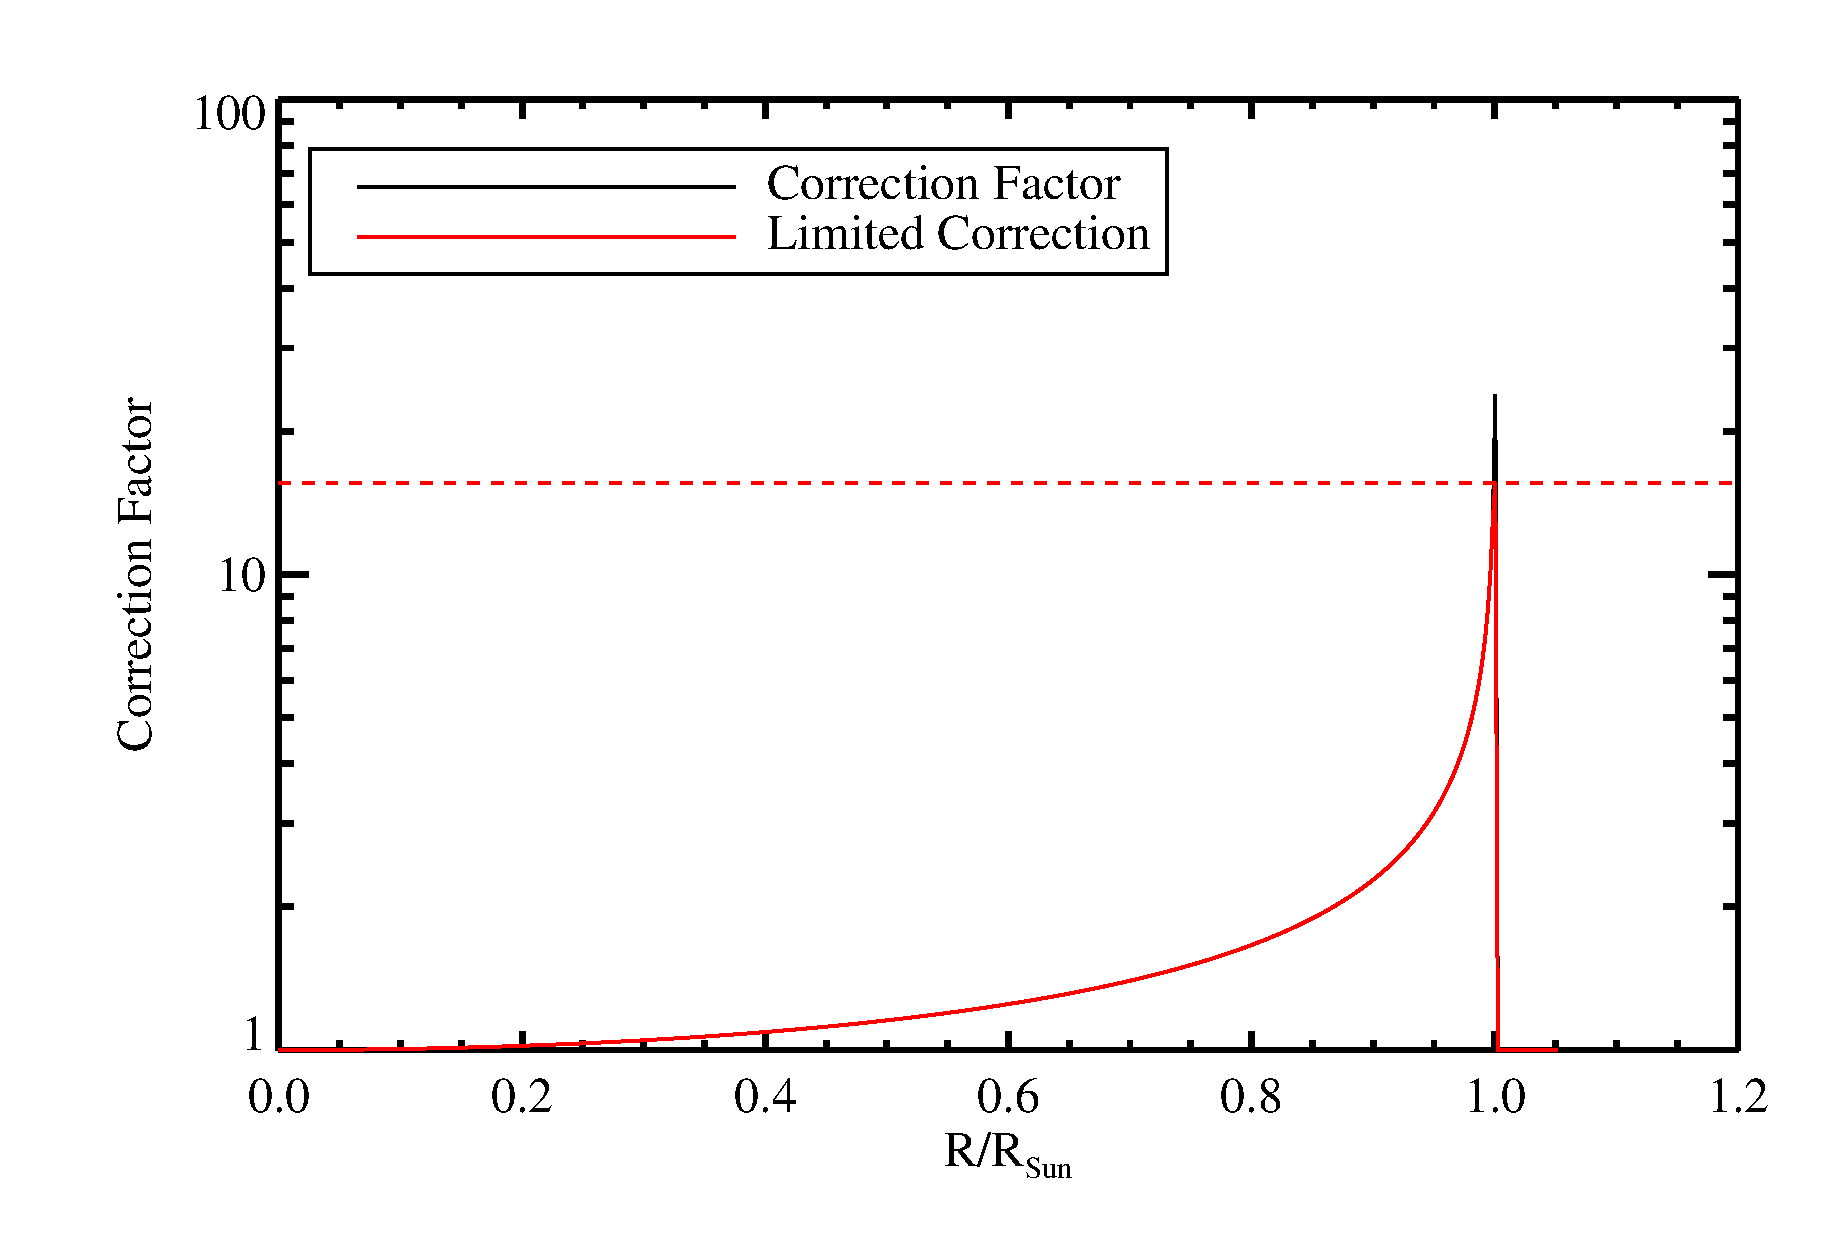
\includegraphics[width=0.9\textwidth,angle=0]{uncert/plot_correction_factor_2.eps}}
\caption[The pixel area LOS correction factor.]{The area cosine-correction factor related to the apparent distance from disk center in solar radii. This is the factor used to determine the deprojected solar surface area covered by a given pixel. The correction factor is limited to $\sim$15, the factor for a pixel at the limb edge.}
\label{fig:areacor}
\end{figure}

The area correction method used is described in Section~\ref{dataproc}. It is a pixel-by-pixel cosine correction factor, where the angle is measured between the normal vector to the solar surface at a given pixel and the \gls{LOS}.
Here we test limiting the correction factor to $\sim$15, that of a \gls{MDI} pixel extending to the limb of the Sun (the maximum correction any pixel would have). A comparison between the limited and non-limited \gls{LOS} correction profiles is shown in Figure~\ref{fig:areacor}. Limiting the correction factor reduces errors in determining the properties of extended magnetic features that reach the solar limb. 

\begin{figure}[!t]
%\begin{center}
%{\renewcommand{\arraystretch}{1}\begin{tabular}{rl}
\centering{
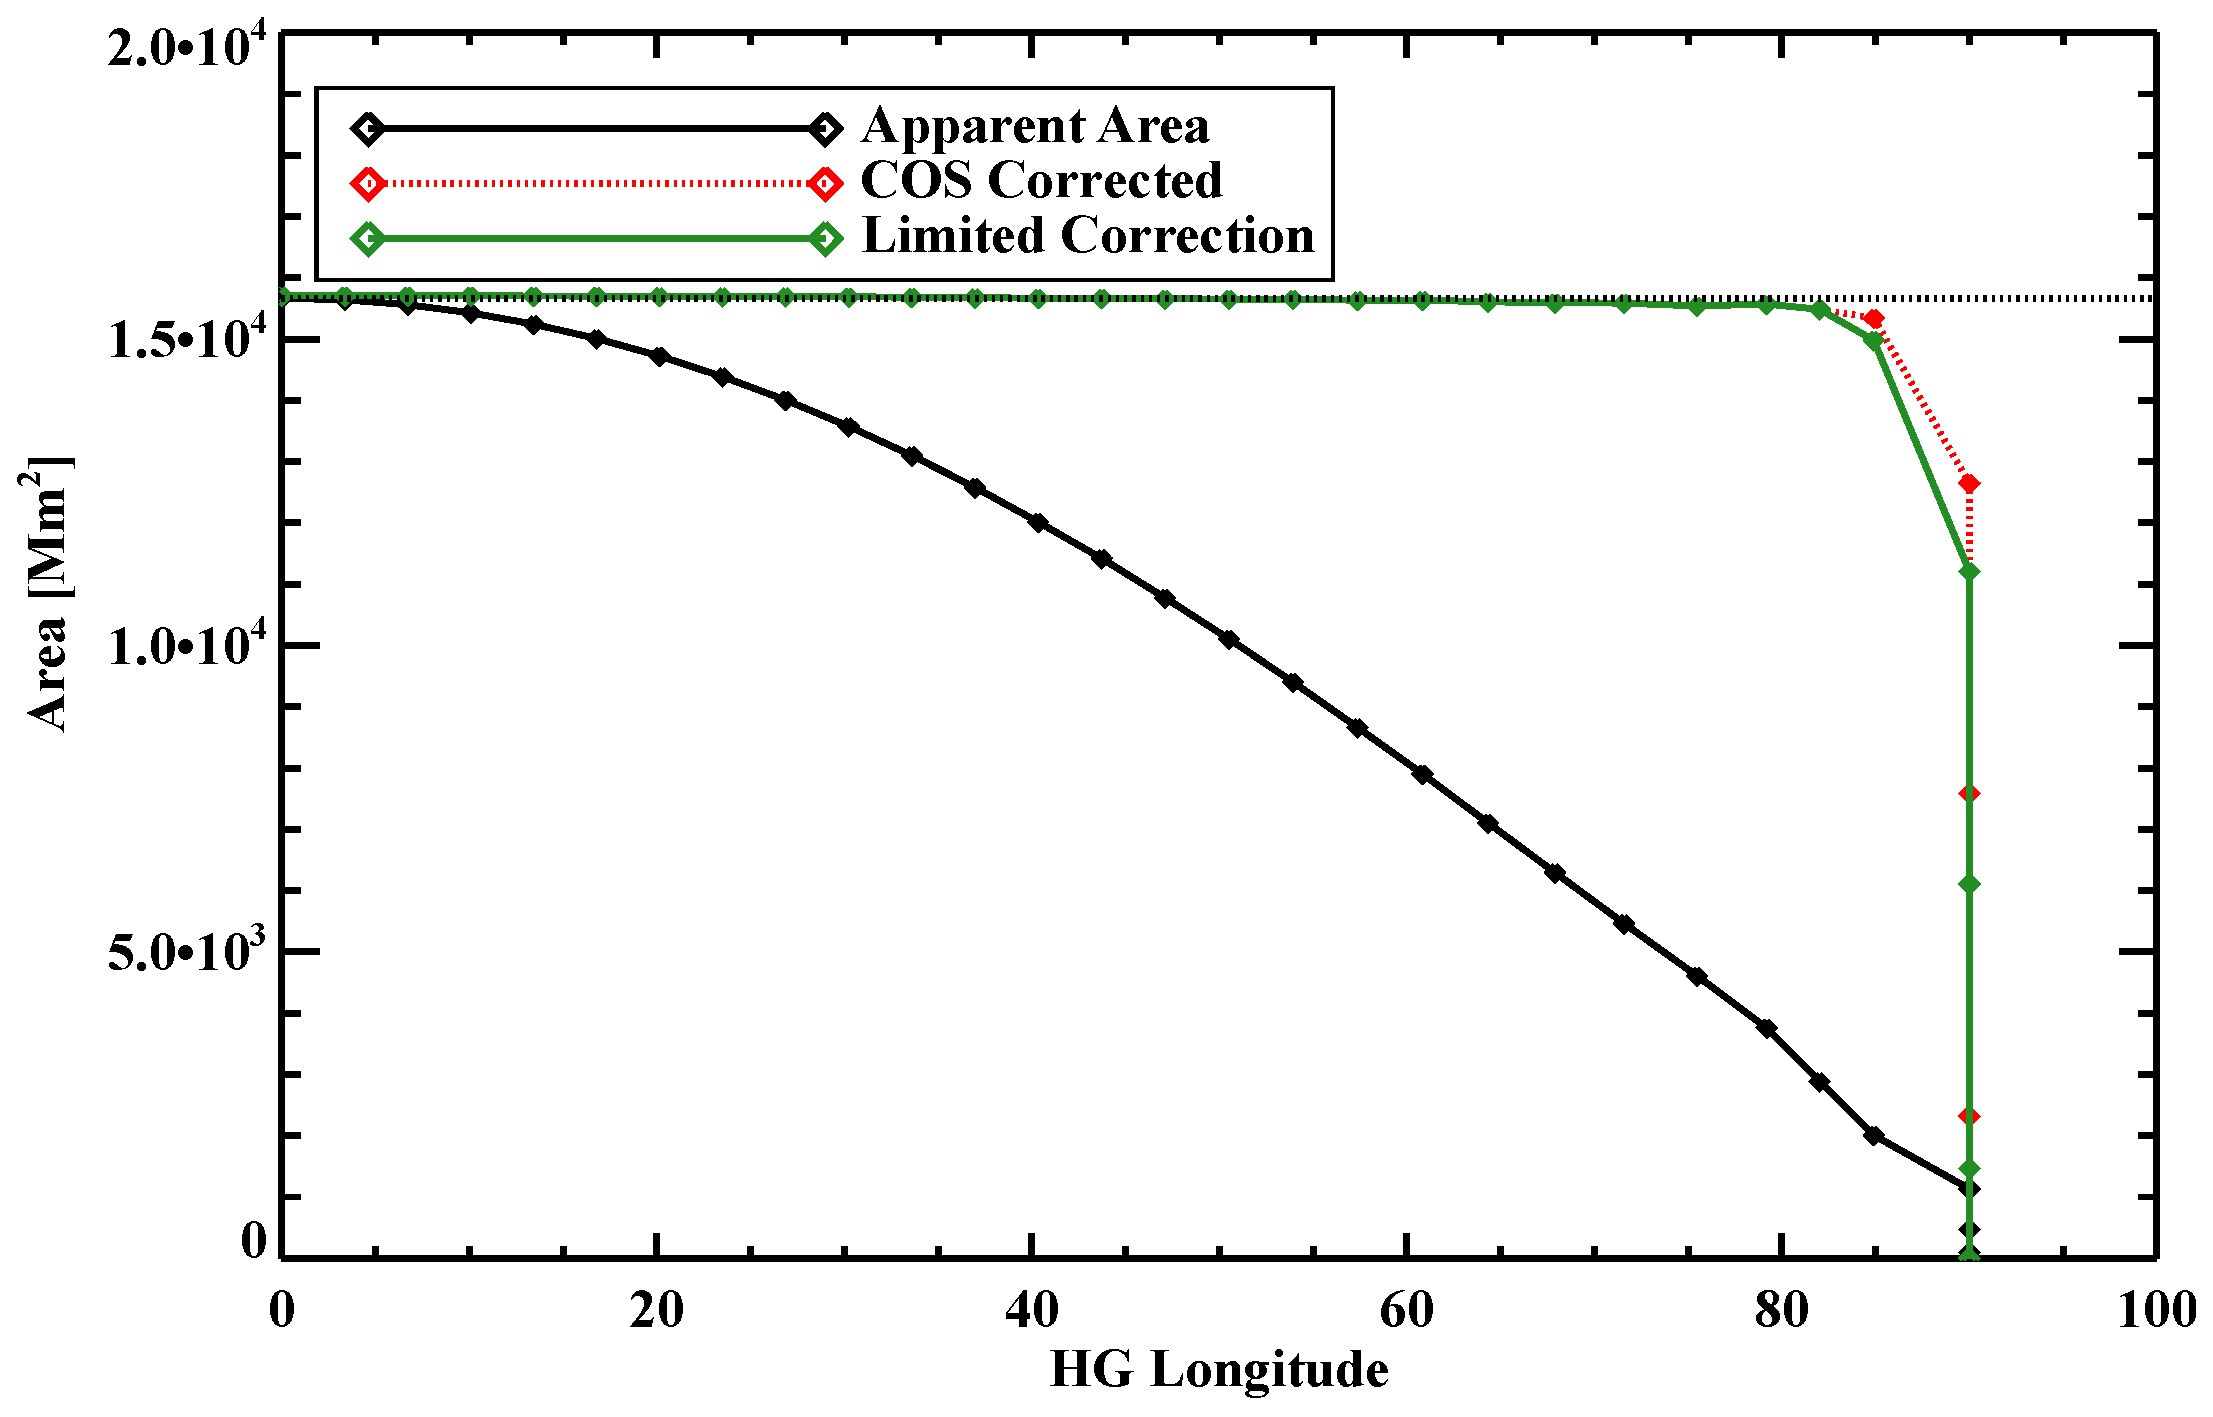
\includegraphics[width=0.8\textwidth,angle=0]{uncert/plot_area_w_correction_vs_hglon.eps} \\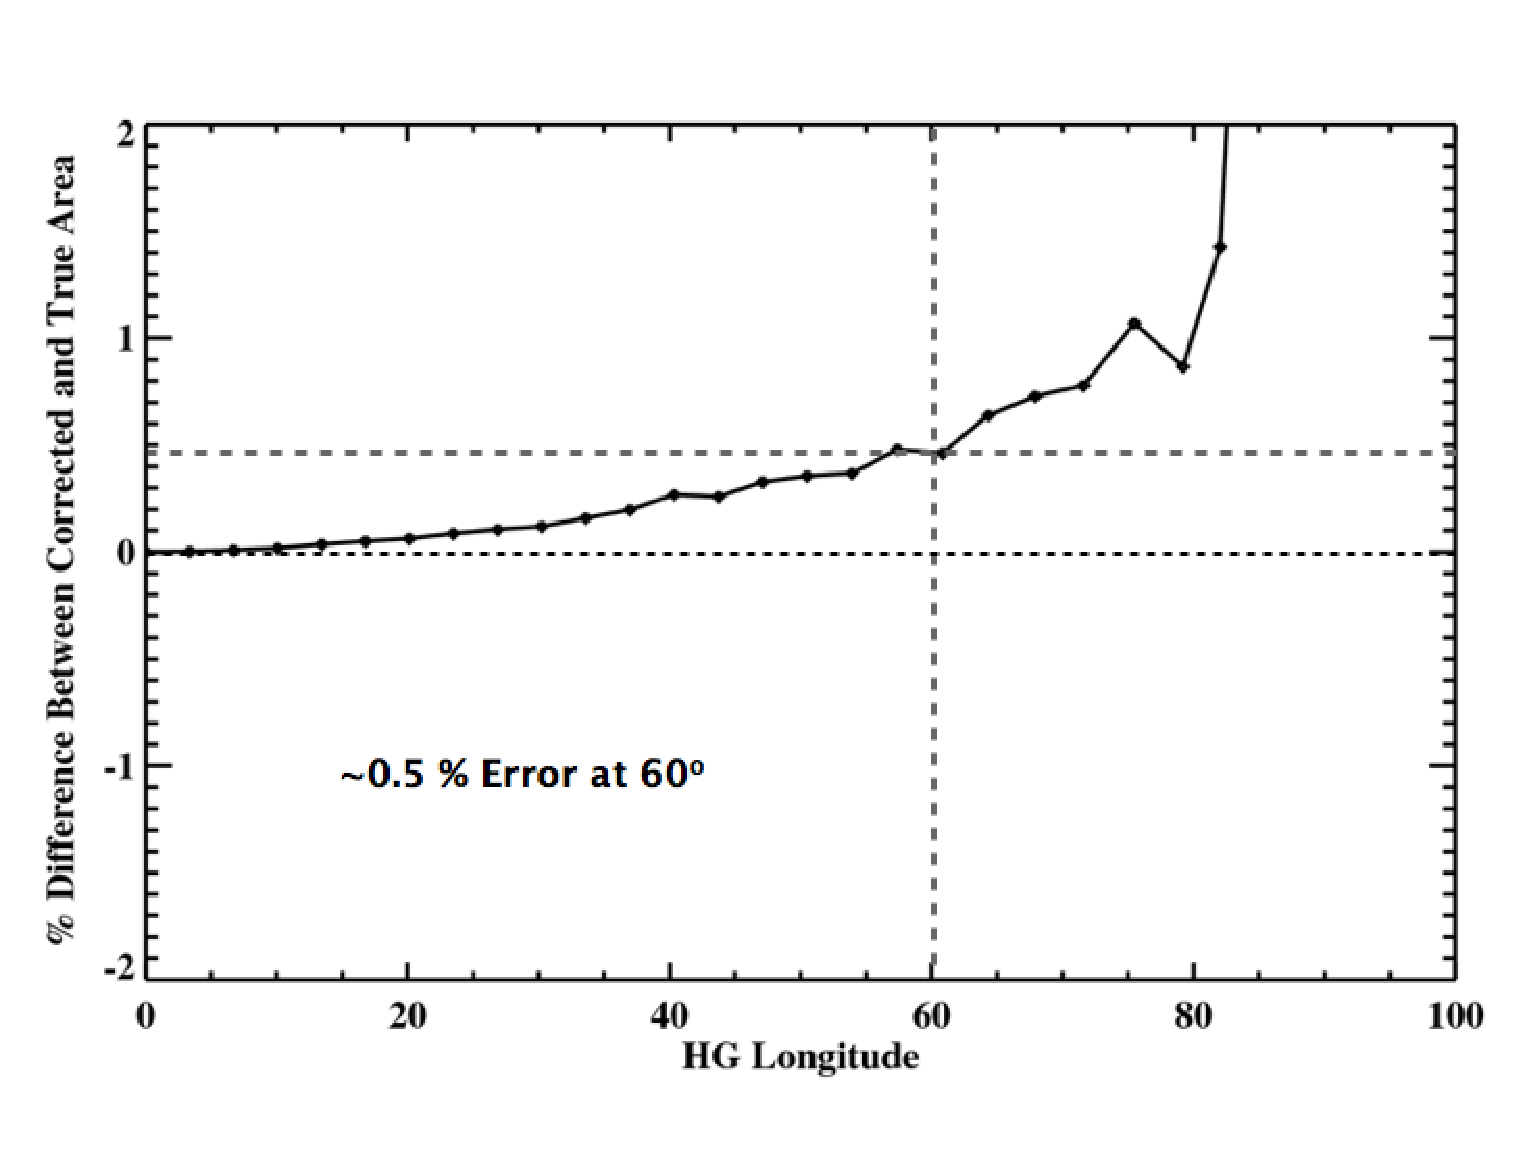
\includegraphics[width=0.8\textwidth,angle=0]{uncert/plot_area_error2.eps}
}
%\end{tabular}}
%\end{center}
\caption[Longitude dependence of area uncertainty.]{The reliability of circular surface feature area measurements with longitude. The top plot shows the apparent area of the circular feature decreasing as it progresses toward the limb. The black dashed line indicates the true area of the feature. The detected cosine-corrected area (red), and the detected area when the correction factor is limited to $\sim$15 (green) are over plotted. The bottom plot shows the \%-difference between the detected area (with the correction limited to $\sim$15) and the true area. The black dashed line indicates the true area and the gray dashed lines indicate the data point at 60$^\circ$ for comparison.}
\label{fig:spotareaerr}
\end{figure}

The comparison between the simulated apparent feature area, cosine-corrected area detected by SMART, and area detected by SMART limited to a correction factor of $\sim$15 is shown in Figure~\ref{fig:spotareaerr}. In this case, limiting the area correction is not important due to the simplicity of the tracked feature. The error in the detected area is shown to be less than 1\% out to $60^{\circ}$ longitude. This error depends on morphology and will be more acute for complex feature boundaries.

\subsubsection{Magnetic Properties of a Bipolar Feature}\label{sect:bipolesim}

\begin{figure}[!t]
\centerline{\includegraphics[width=0.9\textwidth,angle=0]{uncert/psl_sim.eps}}
\caption[A bipole feature disk-crossing simulation.]{A simulation of a magnetic bipole feature crossing the solar disk. Bipole connecting lines are indicated by the red lines in the bottom panels.}\label{fig:bipolesim}
\end{figure}

The superposition of a positive and negative 2D gaussian is used to simulate a bipolar magnetic feature crossing the solar disk. The \gls{FWHM} of the gaussians is $\sim$30\,Mm and the maximum magnetic field is 3\,000\,G. These values are meant mimic a typical sunspot group. This is a simplified representation of a compact magnetic bipole with a trailing high latitude negative sunspot and a leading positive sunspot, tilted toward the equator. The methods of projecting the feature onto the solar disk and simulating differential rotation are the same as that described in Section\,\ref{sect:spotsim}. In addition to area, we determine the total flux, horizontal magnetic gradient and inclination angle of the \gls{PSL} with respect to the \gls{BCL}. Sections\,\ref{magprop} and \ref{sect:char2} describe the methods of determining these detected properties. Figure\,\ref{fig:bipolesim} shows the resulting bipole simulation with the apparent \gls{LOS} projections in the top panels for disk center (A) and near the limb (B). The bottom panels (C and D) show the deprojections of the images into latitude-longitude space. Some distortion is observed at the west-ward edge of the deprojection in panel D, which is because latitude-longitude space becomes increasingly non-conformal\footnote{Conformal projections mean that features keep their shape, while non-conformal projections result in stretching.} near the limb. The deprojected images are only used to determine the PSL and BCL orientation angles, so the distortion will not affect the area and flux measurements.

\begin{figure}[!t]
\centering{
%\begin{tabular}{rl}
\includegraphics[width=0.8\textwidth,angle=0]{uncert/psl_area_hglon2.eps} \\\includegraphics[width=0.8\textwidth,angle=0]{uncert/psl_flux_hglon2.eps}
%\end{tabular}
}
\caption[Plots of corrected area and flux.]{Plots of the apparent (black) and detected corrected area (green; \emph{top}) and detected total flux (\emph{bottom}). The horizontal dashed lines in each plot represent the true values of the properties.}
\label{fig:bipoleareaflux}
\end{figure}

The area of the bipole is determined by creating a mask of the feature using a threshold of 70\,G. This is the threshold used in Section~\ref{dataproc} to detect magnetic features. The area is then corrected as described in Section~\ref{sect:spotsim}.  Likewise the total magnetic flux is summed within the masked region. Since the simulation does not include a cosine decrease of the field with longitude (the fields are all simulated to be normal to the solar surface), only a correction for the area is needed. The detected area and flux exhibit a $\sim$6\% error at $60^\circ$ longitude. The main source of the error is the over-estimation of area due to the shape of the feature \gls{PSL} ends; the detection boundary has two dents, as shown by the white outline in panels A and B of Figure\,\ref{fig:bipolesim}. These dents become less resolved and the detection boundary appears more smooth when the simulated feature is near the limb. 

\begin{figure}[!t]
\centerline{\includegraphics[width=0.7\textwidth,angle=0]{uncert/psl_grad_hglon2.eps}}
\caption[Longitudinal dependence of magnetic gradient.]{The longitude dependence of maximum (black) and mean (green) magnetic field gradient. The horizontal dashed lines indicate the true values of each property.}
\label{fig:bipolegradient}
\end{figure}

The measurement of gradient is performed as described in Section~\ref{magprop}. The error in gradient increases rapidly as the bipole progresses toward the limb. This is not surprising as the apparent separation between the two polarities decreases, while the field strength is constant. The error at $30^\circ$ is already significant at $\sim$15\%. Any statistical study of sunspot group properties using gradients will be strongly affected by the line-of-sight dependence of the observations.

\begin{figure}[!t]
\centerline{\includegraphics[width=0.7\textwidth,angle=0]{uncert/psl_rotation_hglon2.eps}}
\caption[The longitude dependence of the BCL and PSL orientation.]{The longitude dependence of the BCL (black; multiplied by $-1$) and PSL (green) orientation. The difference in orientation between the BCL and PSL is plotted in red.}
\label{fig:bipolerotation}
\end{figure}

The \gls{PSL} is detected using the method described in Section~\ref{magprop}. The error in the measurement of \gls{BCL} inclination and \gls{PSL} inclination are not strongly dependent on longitude. The errors in these inclinations range between 5\% and 15\%. The \gls{BCL} orientation varies smoothly but the \gls{PSL} orientation appears to vary randomly. The main source of the error in this simulation is likely due to the use of gaussians, which result in very small \gls{PSL} detections. Detecting the orientation of a line defined by only a few pixels is highly sensitive to the deprojection interpolation.

This simulation assumes that the fields in the bipole are perfectly radial and that we have corrected the fields perfectly. The uncertainty introduced by inclined penumbral fields has not been accounted for. When determining the flux of a sunspot at disk center, we will be underestimating the fields since there will be only a very small \gls{LOS} component of the penumbral field. Toward the limb, false \glspl{PSL} may be introduced as the horizontal penumbral fields dip below the plane of sky and are measured as the opposite magnetic polarity to their true value at the solar surface. This causes a large error in any property determination using the horizontal field gradient.


%%%%%%%%%%%%%%%%%%%%%%%%%%%%%%%%%%%%%%%%%%%%%%%%%
\section{Conclusions}\label{sect:smartconc}
%%%%%%%%%%%%%%%%%%%%%%%%%%%%%%%%%%%%%%%%%%%%%%%%%

In this chapter, the \gls{SMART} method is described and characterised. It is run on a large magnetogram data set, is benchmarked against another detection method, and its performance is tested using simulated data sets.
%First, the utility of \gls{SMART} is discussed. Then, uncertainties due to the nature of the observations used are discussed. Then uncertainties due to the detection algorithm itself are explained.
\begin{itemize}
\item \gls{SMART} is the first completely automated magnetic feature detection algorithm that detects, characterises, and tracks surface features over multiple solar rotations.
\item The use of MDI \gls{LOS} magnetograms leads to certain situations in which \gls{SMART} results are unreliable, such as determining magnetic properties away from disk centre that involve gradients.
\item The detection and tracking method is stable in time and its use results in a similar representation of the sunspot cycle to that obtained from \gls{NOAA} results.
\end{itemize}
The following sections provide more detail on these points.

\subsection{The SolarMonitor Active Region Tracker}

The \gls{SMART} algorithm allows one to monitor \glspl{AR} on the solar disk in near-realtime and perform extensive studies of \gls{AR} magnetic properties. \gls{SMART} is unique among automated \gls{AR} extraction algorithms in that it allows the temporal analysis of magnetic properties from emergence and through multiple solar rotations. %Future work will include the analysis of trends in \gls{AR} evolution over the solar cycle. This is a largely untouched subject that begs important questions, such as whether \glspl{AR} are born destined to flare or randomly evolve to become flare-active. This may also provide new insights into the behavior of the solar dynamo.
Previous algorithms include some of the functions performed by the
\gls{SMART} algorithm, such as feature and magnetic parameter extraction. However,  new utilities are incorporated into \gls{SMART}, such as day-to-day and multiple rotation feature tracking. Extensive \gls{AR} properties such as area ($A_{tot,t,i}$) and total magnetic flux ($\Phi_{uns,t,i}$) are determined, as are intensive properties such as the maximum magnetic field ($B_{max,t,i}$) and statistical moments ($\mu,\sigma^2,\gamma,\kappa$). Some algorithms, including \citet{LaBonte:2007} only detect the largest regions, while others like \citet{Colak:2009} only detect \glspl{AR} with sunspots in white-light images. All current algorithms track \glspl{AR} using visually identified \gls{NOAA} specifications. The \gls{SMART} algorithm is independent from these specifications and needs no human intervention to detect and track \glspl{AR}. Additionally, it utilizes an improved feature cataloging system which incorporates the date of first detection and the feature type\footnote{Incidently, this cataloging system is very similar to the SOL number presented by Schrijver \emph{et al.} in \url{http://spd.aas.org/SolarNews/archive/news.2009/15.aug} and can easily adapted to match its structure.}.

%The \gls{SMART} algorithm will be used to create a comprehensive catalog of features present in magnetograms covering the entirety of solar cycle 23 and will be adapted to use \emph{SDO}/Helioseismic and Magnetic Imager\footnote{See: http://hmi.stanford.edu} data. A pipeline version of the algorithm will output detections for inclusion in the Heliophysics Event Knowledgebase\footnote{See: http://www.lmsal.com/helio-informatics/hpkb/index.html}. Additionally, it will form part of HELIO. In this application, \glspl{AR} tracked using \gls{SMART} will be associated with a chain of features and events propagating throughout the heliosphere, such as EUV loops, flares, CMEs, magnetic disturbances and storms detectable in Earth's aurorae and ground-based magnetometer data, as well as distant particle instruments such those on the Voyager and Mercury Surface, Space Environment, Geochemistry, and Ranging (\emph{MESSENGER}) spacecraft. 

%The magnetic properties of \glspl{AR} retrieved by the \gls{SMART} algorithm will also be used for flare forecasting. While the magnetic complexity of \glspl{AR} is known to be an important predictor of flare activity \citep{SZT00,Shj07,McAt05b,Con08}, recent work by \citet{Wel09} shows  that extensive magnetic properties outperform intensive properties as predictors of \gls{AR} flare activity. One of SolarMonitor's current flare-forecasting algorithms assumes Poisson statistics \citep{Mn01,Wh01,Gal02} and relies on historical  flaring rates from 1988 to 1996 for each McIntosh sunspot classification \citep{McIn90}. This will be superseded by a statistical forecasting algorithm that makes use of extensive \gls{AR} magnetic properties determined by \gls{SMART}.

\subsection{Observational Uncertainties}

The studies presented in this chapter show that the combination of \gls{MDI} magnetograms and automated detection methods cannot be used to reliably determine the true magnetic field of the Sun. Several sources of error accumulate to result in data products that can only indicate the order-of-magnitude of the magnetic field. These sources of error are a result of the MDI instrument design, calibration, the physical structure of sunspots, and the automated methods used to detect them as discussed throughout this chapter. 

The \gls{MDI} instrument performs a sparse sampling of the Ni\,I spectral absorption line. This leads to strong magnetic fields being less trustworthy, as the Zeeman splitting becomes more complex. Since only \gls{LOS} magnetic fields are measured, complicated magnetic field geometries, such as those in \glspl{penumbra}, are poorly measured. The use of onboard \gls{MDI} data processing has resulted in large errors within strong \glspl{penumbra}. Weak fields measured in the quiet Sun suffer from the significant (nominally) 20\,G noise of the instrument. However, plage fields are high enough above the noise level and low enough below the saturation level and should be, at the least, linear. 

With these problems in mind, it is sensible to ask why \gls{MDI} is used in this work. The instrument covers more than an entire solar cycle, allowing for long time-scale studies. The time coverage is extremely stable, with $\sim$15 evenly spaced images available per day, save for the period at the end of 1998 when \gls{SOHO} was out of contact. The instrument does not suffer from the seeing, weather, and night-time that ground-based instruments must deal with\footnote{There is a whole-earth observatory that produces magnetograms, but seeing conditions vary wildly at each observing location.}. So, \gls{MDI} is very useful for statistical studies of sunspot group properties, as the regimes over which the properties are reliable are predictable.

\subsection{Method Uncertainties}

The automatic detection and characterisation algorithm, \gls{SMART}, is shown to have very good stability in tracking features through time. This indicates that while the algorithm diverges from the detection and tracking behavior of \gls{NOAA}, it is very useful for performing studies of the evolution of sunspot group properties. 

With regards to physical properties, we have shown that flux values are more useful than magnetic field values since flux is conserved, while the magnetic field is averaged over a pixel. Also, the properties determined for features with more complex morphologies are less reliable away from disk center than those with simple morphologies. The gradient values are especially problematic away from disk center. Despite this, near disk center they are extremely useful as flare indicators, as will be shown in Chapter~\ref{chapter:results_activity}.

Any future flare forecasting algorithm which makes use of magnetic properties output by \gls{SMART} will need to take into account several sources of error. Random errors including magnetogram noise and algorithm stability for the example presented in Section~\ref{sect:smartmethuncert} result in an error of $\pm5\%$ and $\pm3\%$ in $\Phi_{uns,t,i}$, respectively. This will not affect the forecasting potential of properties involving ${\Phi}_{uns,t,i}$ for a sufficiently large sample of regions. Calibration errors in MDI result in an underestimate of the true magnetic field on average by $\sim$$30\%$. If the forecasting training set and test samples both exhibit this error, the prediction result will not be affected. However, for physical studies of energetics this must be taken into account. Finally, \gls{LOS} effects which occur as regions approach the limb cause large measurement errors past $60$ heliographic degrees from disk center, which limits the potential flare forecasting range of this algorithm. 

% ---------------------------------------------------------------------------
% ----------------------- end of thesis sub-document ------------------------
% ---------------------------------------------------------------------------